\section{Driedimensionale stapelproblemen}
In de voorbije lessen, hielden we ons bezig om cirkels op een zo optimaal mogelijke manier te stapelen in een driehoek, rechthoek, cirkel ...
Als we dit probleem veralgemenen naar het driedimensionaalgeval, dan krijgen we het zogenaamde probleem van Kepler, waarbij we dus zoeken naar de dichtste bolstapeling.

\subsection{Kanonskogels stapelen}

\begin{wrapfigure}[10]{r}{0.3\textwidth}
  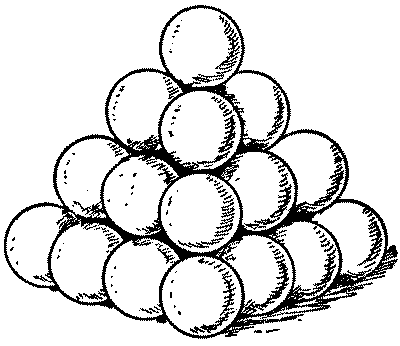
\includegraphics[width=0.3\textwidth]{cannonballs}
\end{wrapfigure}

Ondanks dat het bolstapelprobleem ook het probleem van Kepler genoemd wordt, ontstond het niet bij Kepler, maar bij de Engelse admiraal Sir Walter Raleigh. Wanneer deze Engelse admiraal naar buiten keek vanuit zijn admiraliteitsgebouw, zag hij steeds piramidevormige stapels bestaande uit kanonskogels.  Deze stapels intrigeerden hem zodanig, dat hij zich op een welbepaalde dag afvroeg hoeveel kanonskogels er in zo'n stapel aanwezig waren. Daarom ging hij ten rade bij zijn wetenschappelijk adviseur, Thomas Harriot, om dit  raadsel voor hem op te lossen. 

Voor deze les gaan we ons wat inleven in de rol van Sir Walter Raleigh. Alleen zullen we nu het niet direct vragen aan Thomas Harriot, maar het zelf onderzoeken.

Bolvormige kanonskogels kun je op verschillende manieren als een piramide op elkaar stapelen. Je kunt bijvoorbeeld beginnen om de eerste laag kogels in een vierkant patroon te leggen, maar ook volgens gelijkzijdige driehoeken is het mogelijk, net als bij de jetons in het vlak of de blikjes/glazen op het dienblad. 
Omdat we toevallig niet voldoende kanonskogels bij de hand hebben, kunnen we knikkers gebruiken om dit uit te proberen (ook tafeltennisballetjes of sinaasappelen zijn geschikt).

\task{Ga op zoek naar de formule voor het aantal kanonskogels in een (regelmatige) piramide met vierkant en driehoekig grondvlak (ook voor cirkelvormig en zeshoekig grondvlak zou je dit kunnen uitproberen) met $n$ lagen. \\
Test dit eerst uit door het zelf uit te testen met knikkers voor 1,2, 3 ... lagen. Vul dit in onderstaande tabel in en probeer hieruit zelf tot een formule te komen. Ga dan eens na hoeveel kogels je moet hebben voor 100 lagen.}

\begin{table}[h]
\centering
\begin{tabular}{l|c|c|c|c|c|c}
Aantal lagen: &&&&&&\\\hline\hline
Driehoek: &&&&&& \\\hline
Vierkant: &&&&&& \\
\end{tabular}
\caption{Aantal knikkers voor verschillende piramides met $n=1,...,6$ lagen}
\end{table}



\answer{Het is nu de bedoeling dat de leerlingen zelf de formule gaan zoeken en vinden door dit uit te testen voor verschillende vormen van grondvlakken en voor verschillende lagen ($n = 1, 2, ... , 6 , ... , 100$). Hiervoor kunnen ze dus gebruik maken van knikkers, waarbij je best ook zorgt voor een ruwe ondergrond of een soort omkadering voor het grondvlak. Ook andere bolvormige voorwerpen kunnen gebruikt worden.
De leerlingen zullen algauw gevonden hebben hoeveel knikkers ze moeten gebruiken voor de verschillende rijen en de tabel als volgt hebben ingevuld.
\begin{table}
\centering
\begin{tabular}{l|c|c|c|c|c|c}
Aantal lagen: &1&2&3&4&5&6\\\hline\hline
Driehoek: &1&4&10&20&35&56 \\\hline
Vierkant: &1&5&14&30&55&91 \\
\end{tabular}
\caption{Aantal knikkers voor verschillende piramides met $n=1,..,6$ lagen}
\end{table}
Ook de formule met de sommen moet zeker mogelijk zijn om gevonden te worden.
\begin{itemize}
	\item Formule bij piramide met driehoekig grondvlak:
	 $$d(n)= \frac{1.2}{2} + \frac{2.3}{2}+\frac{3.4}{2} + \cdots + \frac{n(n+1)}{2}$$
	\item Formule bij piramide mert vierkant grondvlak: \[v(n)=1^2 + 2^2 + \cdots + n^2\]
\end{itemize}
}

\task{Test met de knikkers als je volgende vragen een positief antwoord kunnen hebben of vermoedelijk fout zijn...
\begin{itemize}
	\item Kan je van een driehoekige stapel van een bepaalde hoogte een vierkante piramide maken, zonder dat je kogels overhoudt?
	\item Kan je van twee stapels knikkers in vierkante piramides een nieuwe vierkante piramide maken? 
	\item Kan je van twee stapels knikkers in driehoekige piramides een nieuwe driehoekige piramide maken?
	\item Kan je van twee stapels knikkers in driehoekige piramides een nieuwe vierkante piramide maken?
	\item Kan je van een combinatie van een driehoekige en vierkante piramides een andere combinatie van een driehoekige en vierkante piramide maken?\\
Opmerking: piramides van ��n verdiep hoog worden niet meegerekend.
\end{itemize}
}

\teacher{
Na deze testfase is het de bedoeling dat we dit klassikaal overlopen en de antwoorden verklaren.}


\subsubsection{Het aantal kanonskogels bij een piramide met vierkant grondvlak}

We zullen beginnen met de vierkante stapeling.
Om bijvoorbeeld een stapel van vier lagen hoog te maken begin je om 16 kogels netjes in een 4 bij 4 vierkant te leggen. Vervolgens leg je daarop een laag van 9 kogels in een 3 bij 3 vierkant, dan een laag met $2\times2=4$ kogels, en ten slotte is er nog plaats voor ��n kogel als top van de piramide. Voor een 'vierkante' stapel van vier lagen hoog heb je dus $16+9+4+1=30$ kogels nodig.
Als je kijkt naar de antwoorden die je in de tabel gevonden hebt, zijn dat eigenlijk telkens de eerste $n$ kwadraten en dus verkrijg je volgende formule:

\[v(n)=1^2 + 2^2 + \cdots + n^2.\]

\ask{Wat is het nadeel van deze formule als jij bijvoorbeeld het aantal kogels in een stapel van honderd lagen wil bepalen?}

\answer{Om het aantal kogels in een stapel van honderd lagen te bepalen moet je dus ook de eerste honderd kwadraten bij elkaar optellen. Dit is wel te doen, maar een nadeel van dit algoritme is dat de hoeveelheid werk afhangt van de hoogte van de stapel. Voor duizend lagen is het minstens tienmaal zoveel werk als voor honderd.} 

We zullen daarom nu een formule afleiden, waarmee je de som van de eerste $n$ kwadraten direct kunt uitrekenen. Het rekenwerk in een formule is vrijwel onafhankelijk van de hoogte van de piramide. Dat is het verschil met het algoritme waarin de kwadraten worden opgeteld. 

Als we het aantal kogels bij een piramide met $n$ lagen voorstellen door $v(n)$. Dan is $v(1)=1$, $v(2) = 5$ en $v(n)= 1^2 + 2^2+ \cdots +(n-1)^2 + n^2 $. 

\ask{Wat merk je op als je verschillen tussen twee opeenvolgende $v(i)$'s bekijkt?}

\answer{We merken op dat de verschillen tussen twee opeenvolgende $v(i)$'s steeds een kwadraat is, namelijk $v(n)-v(n-1)=n^2$.}
We willen proberen om nu een eenvoudigere formule te vinden voor $v(n)$, een functie die afhangt van $n$, waarbij we dus ook rekening houden met bovenstaande opmerking. Omdat er in de formule 
\[v(n) = 1^2 + 2^2+ \cdots +(n-1)^2 + n^2 \]
enkel kwadraten in voorkomen, kunnen we eens proberen als een kwadratische functie zou kunnen. 

Stel bijvoorbeeld
$$ v(n) = an^2+bn+c.$$
Als dit klopt, dan moet er gelden dat 
\begin{align*}
n^2&=v(n) - v(n-1)=(an^2+bn+c) - (a(n-1)^2+b(n-1)+c)\\
&= (an^2+bn+c) - (an^2-2an)  - (bn-b)-c=2an+(-a+b).
\end{align*}

\ask{Is het mogelijk om hieruit een formule voor $v(n)$ te vinden? Waarom wel/niet?}

\answer{
Je ziet dat helaas de term $an^2$ wegvalt. Er blijft geen kwadratische term over, dus we krijgen het zo nooit voor elkaar om voor elke $n$ waarde $n^2$ uit te komen
In het rechterlid staat iets lineair, in het linkerlid iets kwadratisch. We kunnen nooit $a, b$ en $c$ vinden die dit in orde maken.We zien hier ook de volgende eigenschap van rijen opduiken: De verschilrij van een kwadratische rij is een lineaire rij.}

Aangezien dit niet werkt, is een volgend idee om voor $v(n)$ een derdegraadsfunctie in $n$ te nemen: \[v(n)=an^3+bn^2+cn+d.\]

Dan valt waarschijnlijk de derdegraadsterm weer weg, maar misschien hou je iets kwadratisch over. Er is nog een ander reden waarom dit niet zo'n vreemd idee is. Het aantal kanonskogels in piramide heeft iets te maken met zijn inhoud. Inhoud is iets driedimensionaal met zoiets als de lengte, breedte en hoogte, die telkens van de orde $n$ zijn, dus zal het aantal waarschijnlijk iets met de derde macht van $n$ te maken hebben. 

\task{Ga nu zelf na op analoge wijze dat deze aanpak inderdaad goed blijkt te werken en probeer via een stelsel de juiste waarden voor $a,b$ en $c$ te vinden.}

\answer{
\begin{align*}
n^2&=v(n)-v(n-1)=(an^3+bn^2+cn+d) -(a(n-1)^3+b(n-1)^2+c(n-1)+d)\\
&= (an^3+bn^2+cn+d) -[(an^3-3an^2+3an-a)+(bn^2-2bn+b)+(cn-c)+d]\\
&= 3an^2+(-3a+2b)n+(a-b+c).  
\end{align*}
In deze formule staat aan de linkerkant $n^2$ en rechts een kwadratische functie in $n$. Als we op zoek zijn naar de formule moeten we er zeker voor zorgen dat de co�ffici�nten van de machten van $n$ in beide leden gelijk zijn. Zo moet dus het volgende stelsel gelden:
\[\displaystyle
   \left\{ 
  \begin{array}{l l}
	1&= 3a\\
    0&= -3a+2b \\
     0&= a-b+c\\    
  \end{array}\right.\]  
  Het oplossen van dit stelsel levert ons de waarden $a=\frac{1}{3}$, $b=\frac{1}{2}$ en $c=\frac{1}{6}$. Er geldt dus dat 
$$v(n)= 1^2 + 2^2 + \cdots + n^2= \sum_{i=1}^{n}i^2= \frac{1}{3}n^3+\frac{1}{2}n^2+\frac{1}{6}n + d.$$ En omdat $v(1)=1=1+d$ is $d=0$.
}

 
We verkrijgen dus het volgende resultaat:
\[ v(n)= 1^2 + 2^2 + \cdots + n^2= \frac{1}{3}n^3+\frac{1}{2}n^2+\frac{1}{6}n .\]
Met deze formule kun je dus eenvoudig uitrekenen voor hoeveel kanonskogels er in een stapel van een bepaalde hoogte gaan. Voor een hoogte van $n=4$ lagen krijg je inderdaad 30 kogels, zoals we al eerder zagen. Voor 100 lagen zijn maar liefst 338350 kanonskogels nodig.


De formule voor het aantal kanonskogels bij een piramide van $n$ lagen hoog met vierkant grondvlak is eigenlijk de som van de eerste $n$ kwadraten. 
Meestal wordt de formule geschreven als \[\sum_{i=1}^{n}i^2=\frac{n(n+1)(2n+1)}{6}. \]

\task{ Reken dit even uit om te zien dat dit inderdaad overeenkomt met de formule die wij reeds vonden.}

\begin{opm}
E�n merkwaardig aspect van deze formule is dat er breuken in staan, terwijl het eindantwoord een aantal is en dus altijd een natuurlijk getal moet zijn. 
Dat dit toch altijd goed uitkomt, ondanks de breuken, kun je zien door de formule te schrijven zoals in de vorige opmerking, namelijk $v(n)=\frac{n(n+1)(2n+1)}{6}$.\\ 
Deze vorm zal het ons eenvoudiger maken om te controleren dat de formule effectief een geheel getal is. We willen aantonen dat $n(n+1)(2n+1)$ deelbaar is door 6, of dus deelbaar is door 2 en door 3.\\
Dat $n(n+1)(2n+1)$ deelbaar is door 2 volgt uit het feit dat elk getal $n$ even is, of anders is $n+1$ het wel. Dit betekent dat $n(n+1)$ altijd deelbaar is door 2. 
Als je nu nog kan aantonen dat $n(n+1)(2n+1)$ altijd deelbaar is door 3, dan weten we dat de formule steeds te schrijven is als een geheel getal.
Stel dat $n$ en $n+1$ niet deelbaar zijn door 3, waarbij de resten bij deling door 3 steeds 1 en 2 moeten zijn. Aangezien $2n+1=n+(n+1)$ geeft dit dus 3 (dus 0) als rest bij deling door 3. Hieruit volgt dat $v(n)$ weldegelijk steeds een natuurlijk getal geeft. 
\end{opm}

\subsubsection{Het aantal kanonskogels bij een piramide met driehoekig grondvlak}

Vervolgens kijken we eens naar een piramide met driehoekig grondvlak, meerbepaald een gelijkzijdige (of regelmatige) driehoek als grondvlak.

Bij het experimenteren daarnet heb je zeker gevonden dat je bij een stapel van vier hoog $10+6+3+1=20$ kogels nodig hebben. Merken we op dat 1, 3, 6 en 10 driehoeksgetallen zijn, ze zijn namelijk van de vorm $\frac{n(n+1)}{2}$. Dit komt omdat je per laag een driehoek bekomt met op de top 1 bol, daaronder 2, daaronder 3 enzovoort tot ten slotte $n$ bollen als we ons bevinden op de grondlaag, en de som van de natuurlijke getallen tot en met $n$ is $\frac{n(n+1)}{2}$

Als je nu dezelfde werkwijze als hierboven toepast, bekom je dat 
\begin{align*}
d(n) &= \frac{1.2}{2} + \frac{2.3}{2}+\frac{3.4}{2} + \cdots + \frac{n(n+1)}{2}=\sum_{i=1}^{n}\frac{i(i+1)}{2}\\
&=\frac{1}{6}n^3 + \frac{1}{2}n^2+\frac{1}{3}n.
\end{align*}

Met deze formule kun je dus eenvoudig uitrekenen voor hoeveel kanonskogels er in een stapel van een bepaalde hoogte gaan. Voor een hoogte van $n=4$ lagen krijg je inderdaad 20 kogels, zoals we al eerder zagen. 

\ask{Hoeveel kanonskogels heb je nodig voor 100 lagen?}

\answer{Voor 100 lagen hebben we deze keer 171700 kanonskogels nodig.}

\task{
Ga op analoge wijze als bij de piramide met vierkant grondvlak tewerk en ga na dat dit effectief de juiste formule is.}

\answer{
Als we het aantal kogels bij een driehoekige piramide met $n$ lagen voorstellen door $d(n)$. Dan is $d(1)=1$, $d(2) = 4$ en $d(n)= \frac{1.2}{2} + \frac{2.3}{2}+\frac{3.4}{2} + \cdots + \frac{n(n+1)}{2}$. We merken op dat de verschillen tussen twee opeenvolgende $v(i)$'s steeds een driehoeksgetal is, namelijk $d(n)-d(n-1)=\frac{n(n+1)}{2}$.
We willen proberen om nu een eenvoudigere formule te vinden voor $d(n)$, een functie die afhangt van $n$. Omdat er in de formule
enkel kwadraten in voorkomen, kunnen we eens proberen als een kwadratische functie zou kunnen. Analoog als bij het geval met de vierkante piramide zie je dat de term $an^2$ wegvalt. Er blijft geen kwadratische term over.\\
Een volgend idee is om voor $d(n)$ een derdegraadsfunctie in $n$ te nemen: $$d(n)=an^3+bn^2+cn+d.$$ Ook hier blijkt dit opnieuw te werken.
\begin{align*}
\frac{n(n+1)}{2}&=d(n)-d(n-1)=(an^3+bn^2+cn+d) -(a(n-1)^3+b(n-1)^2+c(n-1)+d)\\
&= (an^3+bn^2+cn+d) -[(an^3-3an^2+3an-a)+(bn^2-2bn+b)+(cn-c)+d]\\
&= 3an^2+(-3a+2b)n+(a-b+c).  
\end{align*}
In het linkerlid staat $\frac{n(n+1)}{2}= \frac{1}{2}n^2+\frac{1}{2}n$. Gelijkstellen van de co�ffici�nten van de machten van $n$ in beide leden geeft ons opnieuw een stelsel:
\[\displaystyle
   \left\{ 
  \begin{array}{l l}
	\frac{1}{2}&= 3a\\
     \frac{1}{2}&= -3a+2b \\
     0&= a-b+c\\    
  \end{array}\right.
  \]  
Het oplossen van dit stelsel levert ons de waarden $a=\frac{1}{6}$, $b=\frac{1}{2}$ en $c=\frac{1}{3}$. Er geldt dus dat 
\begin{align*}
d(n) &= \frac{1.2}{2} + \frac{2.3}{2}+\frac{3.4}{2} + \cdots + \frac{n(n+1)}{2}=\sum_{i=1}^{n}\frac{i(i+1)}{2}\\
&=\frac{1}{6}n^3 + \frac{1}{2}n^2+\frac{1}{3}n+d.
\end{align*}
Omdat $d(1)=1=1+d$ is $d=0$ en krijgen we het gezochte resultaat.
}

\subsubsection{Combinaties van bepaalde piramides}
We weten nu hoeveel kogels er nodig zijn om een \textquoteleft driehoekige' of \textquoteleft vierkante' piramide van kogels te stapelen. We gaan nu op zoek naar de antwoorden op de vragen over het combineren van bepaalde stapels knikkers in de vorm van piramides.

\ask{Is het nu mogelijk om van een driehoekige stapel van een bepaalde hoogte een vierkante piramide te maken, zonder dat je kogels overhoudt?} 

Als je kijkt naar het lijstje, dat we vroeger reeds maakten, met de aantallen die nodig zijn voor een driehoekige, vierkante en zeshoekige piramide, dan zie je dat dit nooit lijkt te kunnen, behalve natuurlijk voor een stapel van ��n kogel hoog.
De aantallen in de driehoekige stapel lijken niet voor te komen in de rij van de vierkante piramides. De tabel kun je nog veel groter maken, maar als er nog steeds geen gelijke getallen voorkomen weet je niet zeker of het nooit gebeurt. Misschien gebeurt het namelijk toch een keer voor een heel er grote stapel. Twee Nederlandse wiskundigen (Frits Beukers en Jaap Top) hebben in 1982 bewezen dat het inderdaad nooit gebeurt, maar het bewijs is te moeilijk om er hier op in te gaan.

\ask{Kan je van twee stapels knikkers in driehoekige piramides een nieuwe vierkante piramide maken?}

\answer{Dit is inderdaad mogelijk.}

\ask{Kan je hiervan een voorbeeld geven?}

\answer{Een driehoekige piramide van 3 lagen en een van 4 lagen bestaan samen bijvoorbeeld uit $10+20=30$ kogels, precies genoeg voor een vierkante piramide van 4 lagen hoog.}

Aan de hand van de verkregen formules kan je aantonen dat dit altijd waar is.

\task{Als je het aantal kogels in een vierkante stapel nog steeds stelt als $v(n)= \frac{1}{3}n^3+\frac{1}{2}n^2+\frac{1}{6}n $ en in een driehoekige stapel als $d(n) =\frac{1}{6}n^3 + \frac{1}{2}n^2+\frac{1}{3}n$, controleer dan dat effectief \[d(n-1)-d(n)=v(n).\]}

\answer{
Als we dit met de formules uitschrijven, krijgen we inderdaad
\begin{align*} 
d(n-1) + d(n)&= \frac{1}{6}(n-1)^3 + \frac{1}{2}(n-1)^2+\frac{1}{3}(n-1)+ \frac{1}{6}n^3 + \frac{1}{2}n^2+\frac{1}{3}n\\
&= (\frac{1}{6}n^3 - \frac{1}{2}n^2+\frac{1}{2}n-\frac{1}{6})+(\frac{1}{2}n^2-n+\frac{1}{2})+(\frac{1}{3}n-\frac{1}{3})+(\frac{1}{6}n^3 + \frac{1}{2}n^2+\frac{1}{3}n)\\
&= \frac{1}{3}n^3 + \frac{1}{2}n^2+\frac{1}{6}n= v(n). 
\end{align*}}

Ten slotte kunnen we ook onderstaande vraag positief beantwoorden.

\ask{Kan je van een combinatie van een driehoekige en vierkante piramides een andere combinatie van een driehoekige en vierkante piramide maken?}

\task{Geef een voorbeeld van zo een combinatie.}

\answer{Een vierkante piramide van 5 lagen en een driehoekige piramide van 4 lagen bevatten samen 65 kogels. Een vierkante piramide van 5 lagen en een driehoekige piramide van 3 lagen bevatten samen ook 65 kogels.}  

\task{Hier zit een algemeen patroon achter. Schrijf deze formule op en probeer deze te bewijzen a.d.h.v. de formule uit vorige opdracht.}

\answer{Uit $v(n)=d(n-1)+d(n)$ halen we dat 
\[ v(n)+d(n+1)=d(n-1) + d(n) + d(n+1) = d(n-1) + v(n+1).\]}

%Snifsnif, dit moet weg :s ...
%\subsection{De hoogte van een stapel kanonskogels}
%We hebben het tot nu toe gehad over het aantal bollen in een piramide, maar hoe zit het met de hoogte? Hoe hoog is bijvoorbeeld een driehoekige piramide van 4 lagen knikkers? Is deze dezelfde als een piramide met een vierkant grondvlak?

%Voor het gemak noemen we de straal van de bollen of kanonskogels of knikkers $r$ en $n$ is opnieuw het aantal lagen. Om de hoogte van de stapel te bepalen is het handig om je te verplaatsen in de positie van de middelpunten van de bollen. 
%Je weet dat de hoogte van de grond tot het middelpunt van de bollen op de onderste laag $r$ is. Ook de hoogte van het bovenste middelpunt tot de top van de piramide is $r$. Als we nu de hoogte weten tussen de middelpunten van twee opeenvolgende lagen, dan hebben we de hoogte gevonden. Het is namelijk zo dat deze hoogtes $h$ dezelfde zijn. De hoogte van de piramide is dan $2r+h$.

%Het komt er nu dus op neer bij de verschillende stapels te zoeken wat de hoogte nu juist is.

%\subsubsection{De hoogte van een stapel met vierkant grondvlak}

%Om de hoogte te bepalen tussen twee opeenvolgende lagen van middelpunt, is het handig om te kijken naar de piramide van 2 lagen. In ons geval is dat dus een piramide van 5 bollen. Kijken we nu naar de middelpunten van deze bollen, dan zien we dat deze opnieuw een piramide vormen. Dit komt omdat de bovenste bol raakt aan de andere vier bollen en daardoor is de afstand van twee middelpunten steeds $2r$. Als we de hoogte weten van deze piramide, dan hebben we het gevonden. 

%\todo{Hier zouden allemaal mooie figuren moeten komen het het aanschouwelijk te maken.
%We kunnen ook gebruikmaken van isomobollen en satestokken die dan de bollen verbinden.}

%De hoogte van de kleine piramide vinden we door twee keer de stelling van pythagoras toe te passen. We bekomen $h=\sqrt{2}r$ als hoogteverschil tussen twee middelpunten. Op die manier vinden we de volgende hoogte van een stapel met vierkant grondvlak en $n$ lagen van bollen met straal $r$:
%$$ r(\sqrt{2}(n-1)+2).$$ 


%\subsubsection{De hoogte van een stapel met driehoekig grondvlak}
%Zo ook kunnen we nu de hoogte berekenen van een stapel met een regelmatige driehoek als grondvlak. In figuur %\ref{tetra} 
%zie je hoe de middelpunten van de bollen een stapel van tetra�ders (regelmatige viervlakken) vormen. Dit komt omdat een bol raakt aan de drie bollen onder zich. Het verbinden van het middelpunt met de 3 andere middelpunten geeft inderdaad een viervlak met zijde $2r$. 
%Op de figuur zien we dat we voor de hoogte van de stapel eerst $r$ omhoog moeten naar een middelpunt van de onderste laag, vervolgens 3 keer de hoogte van een tetra�der en ten slotten nog ��n straal omhoog en we zitten boven op de bovenste bal. De hoogte van de stapel met vier lagen ballen is dus $2r+3h$ waarbij $h$ de hoogte van een viervlak is. Voor $n$ lagen met bollen moeten we $n-1$ lagen tetra�ders omhoog.

%\begin{figure}[h]
%\includegraphics[width=\columnwidth]{tetra}
%\caption{Twintig bollen in een driehoekige piramide en tien tetra�ders gevormd door de middelpunten}
%\label{tetra}
%\end{figure}

%Nu moeten we dus enkel nog op zoek gaan naar de hoogte van zo een tetra�der.
%Beschouw figuur %\label{tetra2}
%De hoogte $h$ van de tetra�der is de lengte van z'n hoogtelijn $TP$. Dat is de lijn die je krijgt door de tetra�der op de tafel te zetten en vanuit het hoogste punt een lijn loodrecht naar beneden te trekken. Het onderste punt $P$ ligt precies midden in de onderste gelijkzijdige driehoek, even ver van alledrie de hoekpunten af. De driehoek $\Delta HMP$ heeft hoeken $30\degree$, $60\degree$ en $90\degree$. Aangezien $r= |HM|= |HP|. \cos(30\degree)=r.\frac{\sqrt{3}}{2}$ vinden we dat $$ |HP|=x= \frac{2}{\sqrt{3}}r.$$

%\begin{figure}[h]
%\includegraphics[width=\columnwidth]{tetra2}
%\caption{}%
%\label{tetra2}
%\end{figure}

%Pas nu de stelling van Pythagoras toe op de driehoek door het geprojecteerde punt $P$, een hoekpunt $H$ van de onderste driehoek en het topje $T$ van de tetra�der, dan
%vind je: $(2r)^2=x^2+h^2$. Samen met de formule voor $x$ vinden we dat de hoogte van een tetra�der met zijden van lengte $2r$ gegeven wordt door $$h=\frac{2}{3}r\sqrt{6}.$$

%De hoogte van een driehoekige piramide van $n$ lagen bollen met een straal van $r$ is dus: $$2r(\frac{\sqrt{6}}{3}(n-1)+1).$$


%\emph{Als de leerlingen in het begin hebben mogen uitproberen met knikkers, kan ook een vraag geweest zijn hoe hoog dat de piramide is van 5 lagen knikkers bij de piramide met een vierkant en met een driehoekig grondvlak. Dit kunnen ze nu ook als opdracht krijgen om effectief uit te rekenen en kijken hoever ze er vanaf zaten.}
%\begin{opdracht}
%Wat is de hoogte van een stapel knikkers gestapeld als een piramide met een vierkant grondvlak van 5 lagen? En hoe hoog is de stapel als het een driehoekig grondvlak zou zijn?
%\end{opdracht}

%\todo{Uitgangspunt cursus}
%\emph{Je kan de leerlingen nog verschillende van deze kleine rekenoefeningetjes geven om te checken desnoods, maar het belangrijskte is dat ze inzien dat er een verschil zit en dat ze zien dat de piramide met $n$ lagen bij een vierkante piramide hoger is dan een piramide met driehoekig grondvlak maar met evenveel lagen. Dit geeft reeds een aanwijzing dat, net zoals in het vlak, de vierkante vulling minder effici�nt is als de honingraatvulling. Dit is dan ook een mooie overgang naar het bolstapelprobleem van Kepler...}

%\todo{De volgende opdracht is een opdracht die ik gewoon overtyp van uit het Zebra-boekje. Zulke opdrachten kan je echter in veelvoud uitvinden ;) ...}
%\begin{opdracht}
%Hoeveel tennisballen met een diameter van 6,5 cm heb je nodig om een driehoekige pirmaide te maken die even hoog is als jezelf? Wegen de ballen samen meer of minder dan jij? Een tennisbal weegt 57 gram.
%\end{opdracht}


\subsection{Het bolstapelprobleem van Kepler}
\subsubsection{Het ontstaan}
\subsubsection*{Thomas Harriot}

\begin{wrapfigure}[7]{r}{3cm}
  \vspace*{-1cm}
  \begin{center}
  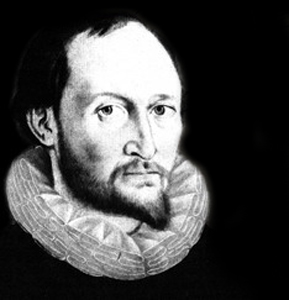
\includegraphics[width=3cm]{harriot}\\
  Thomas Harriot
  \end{center}
\end{wrapfigure}

Je kon al lezen dat Thomas Harriot (1560-1621) door Sir Walter Raleigh (1554-1618) aan het probleem van de piramidestapels werd gezet. Hij was in die tijd als amateur-astronoom bezig met het waarnemen van zonnevlekken en kometen, maar daarnaast was hij ook een bekende wiskundige en dankzij de kennis die hij als wiskundige had, kon hij het probleem van Raleigh in een wip oplossen. Maar nadat hij de oplossing geleverd had, bleef het kanonskogelprobleem in zijn hoofd rondspoken en hij raakte over dit onderwerp in correspondentie met Kepler.

Kepler, die we straks verder zullen bespreken, had al een tijdje een levendige correspondentie met Harriot over het lichtbrekingsverschijnsel. Hij was dan ook niet verbaasd toen hij een briefje kreeg van Harriot. Maar toen hij las dat het over het stapelen van bolvormige voorwerpen ging, werd zijn nieuwsgierigheid aangewakkerd. Niet veel later kwam plots de gedachte bij hem op, om aan de hand van bolstapelingen de structuur van sneeuwkristallen te verklaren. En zo verhuisde het bolstapelprobleem definitief van de gedachten van Thomas Harriot naar die van Johannes Kepler.

\subsubsection*{Johannes Kepler}

\begin{wrapfigure}[9]{l}{3cm}
  \vspace{-10mm}
  \begin{center}
  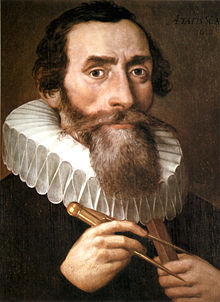
\includegraphics[width=3cm]{kepler}\\
  Johannes Kepler
  \end{center}
\end{wrapfigure}

Kepler (1571-1630) was een beroemde Duitse sterrenkundige die vooral bekendheid kreeg, toen hij aan de hand van de bewegingen van de planeten een beschrijving maakte van hun ellipsvormige banen. Vanaf 1609 onderzocht hij tien jaar lang hoe de afstand van een planeet tot de centrale ster, de omlooptijd en de omloopssnelheid van die planeet be�nvloedde. Dit zou een halve eeuw later opgenomen worden in de zwaartekrachtwetten van Newton. Maar Kepler was niet alleen een beroemde astronoom, hij leverde ook een belangrijke bijdrage tot de wiskunde.

\vspace*{5mm}

In 1611 schreef Johannes Kepler, dankzij de plotselinge inspiratie die hij kreeg door een briefje van Harriot, een boekje met de titel \textquoteleft De zeshoekige sneeuwvlok'. Daarin beschreef hij verschillende methoden om identieke bolvormige voorwerpen in drie dimensies te pakken en hieruit kwam hij tot de conclusie dat de "face-centred cubic packing" de meest effici�nte pakkingsmethode was, waarbij het minst open ruimte tussen de identieke bolvormige voorwerpen overbleef. In het citaat dat hierop volgt beschrijft Kepler zelf wat de "face-centred cubic packing" is.

\begin{quote} "Op de tweede manier wordt niet alleen ieder partikel geraakt door zijn vier buren in hetzelfde vlak, maar ook door vier in het vlak erboven en vier eronder, zodat hij in totaal door twaalf wordt geraakt, en onder druk worden bolvormige partikels rombo�daal(=ruitvormig) ... De pakking zal de dichtst mogelijke zijn, zodat met geen andere rangschikking meer partikels in hetzelfde vat kunnen worden gepakt."  
\end{quote}

Nadat Kepler echter dit vermoeden geleverd had, vond hij het niet meer nodig om hiervoor een bewijs te leveren. En hierdoor bezorgde hij de wiskundigen een probleem dat hen veel bloed, zweet en tranen zou kosten. Maar na bijna 400 jaar zwoegen, zou 'het probleem van Kepler' uiteindelijk bewezen worden. Aangezien het zo lang duurde voordat men tot een bewijs kwam, is het zeker de moeite waard om eens te kijken wat er tijdens die 400 jaren met het probleem van Kepler gebeurde. We zullen dan ook eerst een schets geven van de evolutie van het bolstapelprobleem, vooraleer het bewijs zelf aan te snijden.

\subsubsection*{Kissing number}

Maar voordat we aan de evolutie van het probleem zal beginnen, willen we eerst nog iets vertellen over het getal 12, aangezien voor dit getal een belangrijke rol is weggelegd. 
Het is niet toevallig dat bij de dichtste bolstapeling die Kepler beschrijft, elke bol geraakt wordt door 12 andere identieke bollen. Het getal twaalf is namelijk het kissing number bij drie dimensies. 

\ask{Wat wordt bedoeld met 'kissing numbers'?}

\answer{Een 'kissing number' is gedefinieerd als het aantal niet-overlappende eenheidssferen dat aan een gegeven eenheidssfeer raakt.}

Andere namen hiervoor zijn bijvoorbeeld 'Newton number' of 'contact number'

\ask{Wat is het 'Kissing number' in ��n dimensie? En in twee dimensies? Teken de situatie}

\answer{In ��n dimensie is het 'kissing number' 2, in twee dimensies 6.}
\begin{figure}[h]
  \centering
  \subfloat[]{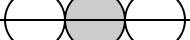
\includegraphics[width= 4 cm]{kissing1}}\qquad
  \subfloat[]{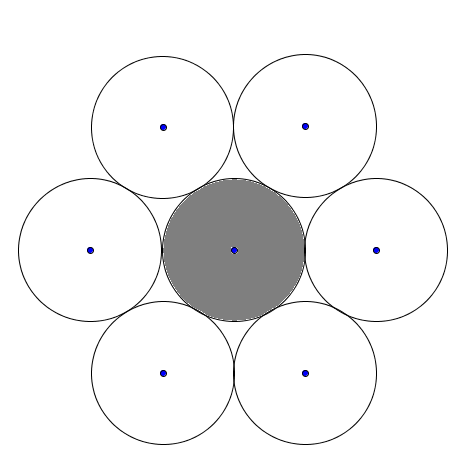
\includegraphics[width= 4 cm]{kissing2}}\qquad
  \subfloat[]{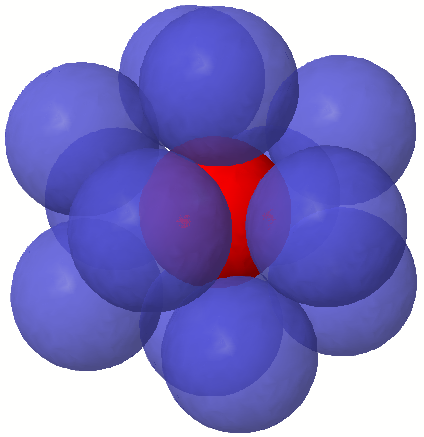
\includegraphics[width=4 cm]{kissing}}
  \caption{Illustraties van kissing number 2, 6 en 12}  
\end{figure}

In het tweedimensionale geval hadden we reeds te maken met dit kissing getal toen we het hadden over het hexagonaal patroon waarbij er dus 6 cirkels de middeltste cirkel raakten.

Over 'kussende getallen', zoals de vertaling luidt, is echter niet zoveel bekend. Men heeft slechts voor vier verschillende dimensies bewezen wat dit effectief getal is en voor de andere dimensies heeft men enkel vermoedens. 

Als we overgaan naar drie dimensies, blijkt dat het kissing number daar dus twaalf is. Concreet wil dit zeggen dat we rond een bolvormig voorwerp slechts 12 andere identieke bolvormige voorwerpen kunnen construeren, waarbij alle twaalf de bollen raken aan deze eerste bol. Wanneer we naar hogere dimensies gaan, wordt onze kennis echter vager. Enkel voor 8 en 24 dimensies is het 'kissing number' gekend. Deze zijn respectievelijk voor 8 dimensies 240 en voor 24 dimensies 196560. Voor de andere dimensies bestaan er boven en ondergrenzen, maar uiteraard is het moeilijk om te vatten hoe we dit ons moeten voorstellen. Voor het bolstapelprobleem is het echter voldoende om te weten wat het 'kissing number' is van drie dimensies.

\subsubsection{Evolutie}

\subsubsection*{De eerste vooruitgang}
Al gauw bleek dat het probleem van Kepler niet zomaar een klein probleempje was dat men in een sneltempo zou kunnen oplossen. Net als bij de laatste stelling van Fermat, bleek het een reusachtig werk om Keplers vermoeden rond het bolstapelen te bewijzen. Dit kwam voornamelijk omdat het bewijs een oneindig aantal mogelijkheden moest omvatten en omdat de wiskundigen dus rekening moesten houden met een enorme reeks verschillende willekeurige bolstapelingen. Zo duurde het dan ook lang voordat men een eerst stap kon zetten in de richting van 'het' bewijs. Maar uiteindelijk na 200 jaar kon Karl Friedrich Gauss een eerste kleinigheid over het vermoeden van Kepler aantonen.
Gauss (1777-1855) was een Duitse wiskundige die zich net als Kepler en Harriot bezighield met astronomie. Gauss er als eerste in slaagde om iets over het vermoeden van Kepler te bewijzen. Hij toonde namelijk aan dat bolstapelingen niet beter konden zijn dan de face-centered cubic packing, wanneer de middelpunten van de gestapelde bollen volgens een vast rooster werden verbonden. Je maakt eerst een laag volgens het gekende hexagonaal patroon en vervolgens leg je er een laag in die je iets verschuift, zodanig dat de bollen net in de kuiltjes van de laag eronder rusten. Bij de volgende laag heb je twee keuzes die niet equivalent zijn. Als we de psoitie van de middelpunten van de bollen in de eerste laaag met $A$ aangeven op de figuur en van de tweede met $B$, dan kan de derde laag precies boven de eerste laag liggen, dus zoals $A$, of op een ander positie, namelijk de $C$ op de figuur. De volgorde met herhaaldelijk $ABC$ wordt die face-centered packing genoemd. Het patroon $AB$ is dan weer dan \textquoteleft Hexagonal Close Packing'. 

\begin{figure}[h]
\centering
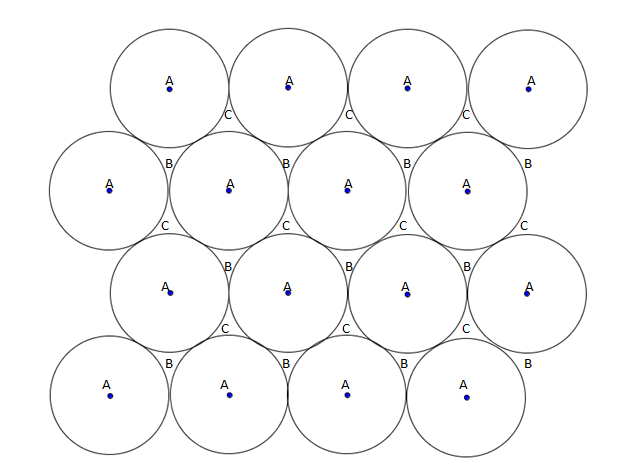
\includegraphics[width=10cm]{fcc}
\caption{Lagen $A$, $B$ en $C$ van de bolsapel}
\end{figure}


Het bewijs voor dit vermoeden bevatte geen berekeningen en was eigenlijk heel kort. Gauss zag dat wanneer 2 bollen elkaar raakten, het rooster ervoor zou zorgen dat een hele rij opeenvolgende bollen elkaar zou raken, waardoor evenwijdige rijen bollen zouden ontstaan. Wanneer deze rijen elkaar raakten, zouden zij het minst ruimte overlaten, als de middelpunten van drie bollen een gelijkzijdige driehoek vormden en zo verkreeg hij een oneindig aantal identieke vlakken met bollen die op de dichtste manier gestapeld waren. Uiteindelijk plaatste hij deze identieke vlakken boven elkaar op zo'n manier dat elke bol in een vlak raakte aan 3 bollen in het vlak erboven en 3 bollen in het vlak er onder. Hiermee verkreeg hij het dichtste bolstapelmodel in drie dimensies volgens een rooster en bewees hij dat de \textquoteleft face-centered cubic packing' de dichtste pakkingsmethode was volgens een rooster. Maar hij toonde hiermee niet aan dat de \textquoteleft face-centered cubic packing' de dichtste pakkingsmethode was van �lle soorten pakkingsmethodes. Op dit bewijs was het nog eens bijna 200 jaar wachten, maar in tussentijd werden wel nog andere dingen in verband met 'het probleem van Kepler' bewezen.

\subsubsection*{Voronoicellen %en Delaunay-sterren
}

In sectie \ref{axel} hebben we het reeds gehad over de Scandinavische wiskundige Axel Thue (1863-1922) die in 1892 een theorie over het tweedimensionale equivalent voor \textquoteleft het probleem van Kepler' waarin men zocht naar de dichtste pakkingsmethode voor cirkels in het vlak. Thue betegelde het vlak met identieke gelijkzijdige zeshoeken en tekende in elke zeshoek een cirkel op zo'n manier dat elke cirkel alle zijden van de zeshoek raakte. Hier werkte hij dus met de zogenaamde Voronoicellen.

Algemeen genomen is dit, zoals je ondertussen wel weet, een ruimtelijk gebied rond een bepaald punt $A$, waarbinnen alle punten dichter bij A liggen dan bij elk ander gegeven punt $B, C, D...$ Dit wil zeggen dat een willekeurig genomen punt in een Voronoicel dichter ligt bij het centrum dat in deze cel ligt dan bij een centrum uit om het even welke andere Voronoicel.
Bij drie dimensies is het construeren van een Voronoicel niet zo eenvoudig. Elke bol heeft een complex omhulsel waarbinnen elk punt dichter ligt tot het eigen bolcentrum dan tot om het even welk ander bolcentrum.
Bij de \textquoteleft face-centered cubic packing' is de Voronoicel een ruitvormige dodeca�der (een regelmatig twaalfvlak). Het vermoeden van Kepler kan dan bijgevolg ook aangetoond worden als men kan bewijzen dat deze ruitvormige dodeca�der de kleinste Voronoicel is bij het bolstapelen.

Deze begrippen spelen een belangrijke rol in het uiteindelijke bewijs van Kepler. Ze zorgen er immers voor dat het reusachtige werk, om de dichtheid van elke bolstapeling te bepalen, wordt beperkt tot een specifieke berekening die uitgevoerd kan worden met de computer. Men zal niet langer zoeken naar de hoeveelheid ruimte die bollen innemen in een stapeling. In de plaats daarvan zal men zoeken naar de kleinst mogelijke Voronoicel.


\subsubsection*{L�szlo Fejes T�th}
De persoon die als eerste suggereerde om Voronoicellen te gebruiken in het bewijs voor het bolstapelprobleem was L�szlo Fejes T�th. Deze Hongaarse wiskundige toonde hiernaast ook aan dat je het vermoeden van Kepler voor oneindig veel bollen kon bewijzen door het voor 50 bollen te bewijzen. Daarnaast ontdekte hij dat er maar 5000 mogelijke stapelingen meer meededen in de strijd om de compactste stapeling. 
T�th wist dat je aan de hand van Voronoicellen kon bewijzen welke van de 5000 stapelingen de grootste dichtheid had. Maar hij ondervond uit zijn onderzoeken dat de grenzen van deze cellen niet voldoende waren, waardoor er een correctieterm moest ingevoerd worden. T�th was de eerste wiskundige die een voorstel deed voor zo'n correctieterm (1953). Alleen bleef toen nog onduidelijk of T�th in zijn berekening met correctieterm alle mogelijke stapelingen had vervat. Het werd wel duidelijk dat Keplers probleem kon opgelost worden met een optimalisatieprogramma met een eindig aantal variabelen en dat dit met de computer zou moeten opgelost worden. Jammer genoeg had men in 1953 nog niet de computers van tegenwoordig, waardoor het nog even wachten was op het uiteindelijke 'bewijs' voor 'het probleem van Kepler'. 


\subsubsection*{Een verlaging van de bovengrens}
In tussentijd probeerden de wiskundigen wel om het vermoeden van Kepler op een andere manier te bewijzen. Zij deden dit door te kijken welke dichtheid er maximaal bereikt kan worden. Indien het hen zou lukken om deze bovengrens te verlagen tot 74.05\%  kon men Kepler bij verstek gelijk geven, aangezien de dichtheid die hij verkreeg \[\frac{\pi}{\sqrt{18}}= 0,74048048\dots\] was. Daardoor zou de grens tussen de dichtheid bij de face-centered cubic packing en de bovengrens zo klein zijn dat er geen betere pakking meer kon bestaan dan de face-centered cubic pakking.
Maar het verlagen van de bovengrens bleek moeilijker dan men dacht. In 1958 behaalde C.A.Rogers een waarde van 77.964\%. Enkele decennia later verkreeg Lindsey in 1986 een bovengrens van 77.844\% en slechts twee jaar later vond Muder een grens van 77.836\%. De meest recente bovengrens verkreeg Muder in 1993, maar die was nog steeds 77.3055\% wat niet zoveel beter was dan de vorige bovengrens en nog steeds ver van hetgeen Kepler vermoedde. 
We kunnen dus concluderen dat het verlagen van de bovengrens niet echt effici�nt was. Daarom gaan we er dan ook niet meer verder op in. 




\subsubsection*{Wu-Yi Hsiang}
Wu-Yi Hsiang is een wiskundige van de universiteit van Californi�, die plots in de zomer van 1988 in de krant verscheen met zijn  bewijs voor het vermoeden van Kepler. Jammer genoeg bleek na een eerste controle dat het bewijs vol blunders zat, waardoor Hsiang zijn werk moest herbekijken. Een jaar later publiceerde hij dan zijn gereviseerde bewijs, maar opnieuw bleken er nog hiaten aanwezig te zijn, waardoor het bewijs nog steeds ongeldig was. Hierna volgde er een lange strijd tussen Hsiang en zijn critici, waarbij argumenten en tegenargumenten voor het bewijs elkaar opvolgden. Maar jammer voor Hsiang aanvaardde de wiskundige gemeenschap het bewijs niet. Ook Thomas Hales die uiteindelijk zelf het bewijs zal leveren vond het bewijs van Hsiang nonsens. Zo blijkt immers uit ��n van de brieven van Hales aan Hsiang, waarin hij schrijft: 
\begin{quotation}"E�n aanname in uw tweede verhandeling treft me als fundamenteler en toch veel moeilijker te bewijzen dan de andere ... U stelt dat 'de beste (dat is: volumeminimaliserende) manier om een tweede laag toe te voegen is zoveel mogelijk gaten af te dekken...' Uw redenering lijkt me zwaar en doorslaggevend op die aanname te steunen, en desondanks zie ik nergens een zweem van bewijs."
\end{quotation}
In 1996 gaf een zekere Doug Muder een samenvatting van de toenmalige situatie rond het bewijs voor het vermoeden van Kepler. Hierin kwam hij tot verschillende conclusies. Ten eerste zei hij dat het geschrift van Hsiang hoogstens een schets is van het vermoeden van Kepler. Ten tweede ontdekte hij dat zelfs deze schets tekortkomingen bevat, doordat enkele wiskundigen meerdere tegenvoorbeelden voor cruciale stappen in het bewijs van Hsiang  gevonden hebben. Als conclusie vindt hij dat het werk rond het Kepler-vermoeden moet voortgezet worden alsof Hsiangs geschrift nooit heeft bestaan.


\subsubsection{Het bewijs voor \textquoteleft het probleem van Kepler'}

\subsubsection*{Thomas Hales en Samuel Ferguson}


\begin{wrapfigure}[7]{l}{3cm}
  \vspace{-10mm}
  \begin{center}
  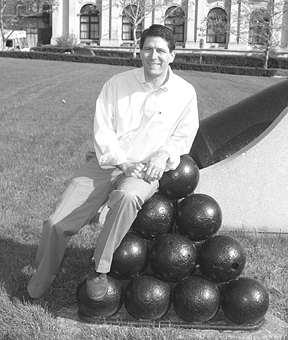
\includegraphics[width=3cm]{hales}\\
  Thomas Hales
  \end{center}
\end{wrapfigure}

Op 9 augustus 1998 kwam het einde voor het bewijs eindelijk in zicht. Thomas Hales, werkzaam aan de universiteit van Pittsburgh, Pennsylvania, stuurde toen een e-mail naar zijn collega's met het opluchtende nieuws dat hij het vermoeden van Kepler bewezen had.
\begin{quotation} "I have started to distribute copies of a series of papers giving a solution to the Kepler conjecture, the oldest problem in discrete geometry." 
\end{quotation} 
Hales toonde Keplers vermoeden aan in een reeks van artikelen die samen het complete bewijs vormen. In totaal gaat dit over 7 artikelen van Hales en een proefschrift van zijn doctoraatstudent, Samuel Ferguson, samen ongeveer 250 pagina's met daarbij 3 gigabytes aan computercode.
Om Keplers vermoeden te bewijzen, steunde Hales op een werk van L. Fejes T�th, waarin staat dat men slechts 5000 stapelingen moet controleren om het vermoeden van Kepler te bewijzen. Hales verdeelde deze 5000 stapelingen in 5 categorie�n waarvan hij er vier zelf bewees. De laatste categorie liet hij over aan Samuel Ferguson.


\subsubsection{Twijfels achteraf}
Ondanks dat alles dus achter de rug bleek te zijn, bleven sommige wiskundigen twijfelen aan de bewijsmethode van Hales. Zij mopperden dat deze brute aanpak met de computer niet echt \textquoteleft interessant' is, omdat men er niets van leert. Er zijn immers geen interessante denkstappen die men kan gebruiken voor andere onderzoeken.
Om de twijfelaars toch te overtuigen werd het gigantische computerprogramma van Hales gecontroleerd door twaalf mensen onder leiding van G�bor Fejes T�th, de zoon van de wiskundige op wie Hales zich baseerde. Na ongeveer 5 jaar kwamen de referees tot de slotsom dat het bewijs zeker voor 99\% klopte.
Maar er bleef toch nog een kleine marge open die twijfel bleef zaaien, waardoor men het bewijs van Hales en Ferguson publiceerde met een kleine kanttekening.

Omdat dit een tegenvaller was voor Hales, startte hij zelf een nieuw project om zijn bewijs formeel te controleren. Hierbij gebruikte hij opnieuw een computer om zijn computerprogramma door te lichten. Hales denkt dat dit project binnen de 20 jaar zal afgerond zijn. Als reactie op Hales zoekactie F*P*K (Formal Proof of the Kepler conjecture) ging ook het project Flyspeck van start.
Collega-wiskundigen spraken hun angst uit dat Hales teveel gebruik maakt van computers. Volgens hen zal de groeiende rol van de computers leiden tot wiskunde die onvatbaar zal zijn voor de mensen. Toch is Hales' bewijs niet de eerste wiskundige krachtmeting van de computer. Het bekendst is waarschijnlijk het vierkleurenprobleem, het probleem dat men minimaal vier kleuren nodig heeft om elke willekeurige landkaart zo in te kleuren dat er geen twee gebieden met dezelfde kleur aan elkaar grenzen. Dit is opgelost door een computerprogramma. Ook in het begin van onze lessenreeks zagen we een bewijs met behulp van de computer, namelijk dat de laagste orde voor een perfect vierkant 21 is.

\subsubsection{Conclusie}
Een eerste punt dat naar voor komt als je de evolutie van het bewijs van Kepler bekijkt, is het feit dat het bolstapelprobleem toch moeilijker is dan het lijkt. Ondanks dat men dus al decennia lang wist dat de face-centred cubic packing de meest compacte stapeling is, kon men dit vermoeden niet bewijzen. Het vermoeden van Kepler bleef dus eeuwen zonder bewijs. Het grootste probleem was het feit dat er enorm veel mogelijke stapelingen zijn, waarvan men niet wist welke nu de meest compacte was. Gelukkige kon Thomas Hales uiteindelijk de wiskundige gemeenschap verlossen met zijn bewijs.
Of toch niet? Want doordat Hales dit probleem met de computer bewezen heeft, laaide opnieuw de discussie op over de rol van de computer in bewijsvoeringen. De ene wiskundige vindt het goed dat er computers gebruikt worden, maar de andere denkt dat we op die manier te veel gehecht gaan geraken aan technologische hulpmiddelen, waardoor wiskundigen geen bewijzen meer zullen kunnen opstellen op de traditionele manuele manier. 

\ask{Wat vinden jullie van een bewijs met de computer?}

Ondanks het bestaan van computers en alsmaar meer kennis blijven er echter nog veel problemen onopgelost. Er zijn nog veel nieuwe interessante dingen te ontdekken en uitdagingen aan te gaan. Daardoor blijft de wiskunde nog zeer actueel en levendig.
